\documentclass[../main.tex]{subfiles}
\begin{document}

In this section we present a formal graph-theoretic framework for truth
discovery, and set out the central problem of truth discovery via the
definition of a \emph{truth discovery operator}. We then develop axioms
(desirable properties) for such operators, and prove some basic properties
regarding them. Finally, we consider how to represent real-world truth
discovery algorithms in the developed framework, focussing specifically on
\emph{Sums} \cite{pasternack}.

First we state some standard definitions and notation.

\subsection{Standard definitions and notation}

\begin{definition}
A \emph{preorder} on a set $X$ is a binary relation $\preceq$ that is reflexive
and transitive:
\begin{enumerate}
\item $x \preceq x$ for all $x \in X$ (reflexivity)
\item If $x \preceq y$ and $y \preceq z$, then $x \preceq z$ for all $x, y, z
\in X$ (transitivity)
\end{enumerate}

A \emph{total preorder} is a preorder that is complete: for all $x, y \in X$,
$x \preceq y$ or $y \preceq x$. $\orderings(X)$ is the set of all total
preorders on $X$.

The \emph{strict} order induced by $\preceq$ is $\prec$ where $x \prec y$ if
and only if $x \preceq y$ but not $y \preceq x$. Note that $\prec$ is
irreflexive, transitive (and hence asymmetric), and is not complete.

The \emph{equality predicate} associated with $\preceq$ is $\simeq$, where $x
\simeq y$ if and only if $x \preceq y$ and $y \preceq x$. Note that $\simeq$ is
an equivalence relation on $X$.

\end{definition}

\begin{definition}
A \emph{permutation} of a set $X$ is a bijective mapping $X \rightarrow X$. We
use cyclic notation for permutations: $\pi=(a, b, c)$ is the mapping $\pi(a) =
b$, $\pi(b) = c$, $\pi(c) = a$, and $\pi(x) = x$ for $x \notin \{a, b, c\}$.
Juxtaposition of cycles denotes function composition.
\end{definition}

\begin{definition}

Two graphs $G=(V, E)$ and $G'=(V', E')$ are \emph{isomorphic} if there is a
bijective mapping $\phi: V \rightarrow V'$ such that $(u, v) \in E \iff
(\phi(u), \phi(v)) \in E'$.

\end{definition}

\begin{definition}
Let $G=(V, E)$ be an undirected graph, and define a relation $\sim$ on $V$ by
$u \sim v$ iff there is a path from $u$ to $v$ in $G$ (including the
zero-length path when $u = v$). It is easily checked that $\sim$ is an
equivalence relation. A \emph{connected component} of $G$ is an induced
subgraph of an equivalence class of $\sim$.
\end{definition}

\begin{notation}
For sets $X$ and $Y$, $Y^X$ denotes the set of all functions $X \rightarrow Y$.
\end{notation}

\subsection{Truth discovery definitions}

We consider fixed finite and mutually disjoint sets $\S$, $\F$ and $\O$, called
the \emph{sources}, \emph{facts} and \emph{objects} respectively. All
definitions and axioms will be stated with respect to these sets.

% Input network definition
\begin{definition}

A \emph{truth discovery network} is a directed graph $N = (V, E)$ where $V = \S
\cup \F \cup \O$, and $E \subseteq (\S \times \F) \cup (\F \times \O)$
satisfies the following properties:

\begin{enumerate}
\item Each $f \in \F$ has a unique successor node in $\O$, denoted $\obj(N, f)$
(i.e. each fact relates to a single object).

\item For $s \in \S$ and $o \in \O$, there is at most one directed path from
$s$ to $o$ (i.e. sources can only claim one fact per object).

\item $(\S \times \F) \cap E$ is non-empty (i.e. at least one claim is made).

\end{enumerate}
We will say that $s$ \emph{claims} a fact $f$ when $(s, f) \in E$. Let $\N$
denote the set of all truth discovery networks.
\end{definition}

\begin{remark}
Note that the definition above does not rule out a source $s$ making no claims,
a fact $f$ being claimed by no sources, or an object $o$ having no associated
facts or sources.

In the special case where each object has exactly two associated facts, the
objects can be seen as \emph{binary variables} taking one of two values, e.g.
true or false. The truth discovery network is then similar to a set of
judgements in \emph{judgement aggregation} \cite{handbook_ja} for an agenda
consisting only of propositional variables.
\end{remark}

\begin{notation}
For convenience, for a network $N=(V, E)$, define:
\begin{align*}
    \fact(N, s) &= \{f \in \F : (s, f) \in E\} \\
    \fact(N, o) &= \{f \in \F : (f, o) \in E\} \\
    \src(N, f) &= \{s \in \S : (s, f) \in E\} \\
    \src(N, o) &= \{s \in \S : \exists f \in \F : (s, f), (f, o) \in E\} \\
\end{align*}
\end{notation}

% Algorithm definition
\begin{definition}
\label{def:truth_discovery_operator}

A \emph{truth discovery operator} $T$ is a mapping $T: \N \rightarrow
\orderings(\S) \times \orderings(\F)$, i.e. $T$ assigns to each truth discovery
network $N$ a pair of total preorders $T(N) = (\sle_N^T, \fle_N^T)$ on the sets
$\S$ and $\F$ respectively.

$s_1 \sle_N^T s_2$ means $s_2$ is ranked as \emph{more trustworthy} than $s_1$
in the network $N$ according to $T$; $f_1 \fle_N^T f_2$ means $f_2$ is ranked
as \emph{more believable} than $f_1$.

\end{definition}

In practise, real-world truth discovery algorithms do not usually output a
ranking of sources and facts directly, but instead assign each source a numeric
\emph{trust score}, and each fact a \emph{belief score}. This is captured in
the following definition.

\begin{definition}
\label{def:numerical}

A \emph{numerical truth discovery operator} $T$ is a mapping $T: \N \rightarrow
\R^\S \times \R^\F$, i.e. $T$ assigns to each truth discovery network $N$
functions $t_N: \S \rightarrow \R$ (referred to as the \emph{source trust}
mapping) and $b_N: \F \rightarrow \R$ (referred to as the \emph{fact belief}
mapping).

\end{definition}

\begin{remark}
    Any numerical truth discovery operator $T$ naturally induces a
    truth discovery operator $T'$, where for any truth discovery network $N$
    we define
    \begin{align*}
    s_1 \sle_N^{T'} s_2 & \iff t_N(s_1) \le t_N(s_2) \\
    f_1 \fle_N^{T'} f_2 & \iff b_N(f_1) \le b_N(f_2)
    \end{align*}
    for $s_1, s_2 \in \S$ and $f_1, f_2 \in \F$.
\end{remark}

In this work we deal primarily with truth discovery operators as defined in
definition \ref{def:truth_discovery_operator}, instead of working directly with
numeric trust and belief scores as in definition \ref{def:numerical}. This is
because, from a theoretical point of view, we are interested in the qualitative
ranking of sources and facts, rather than quantitative values. This approach is
common in axiomatic treatment of social choice and ranking systems
\cite{handbook_voting,arrow,altman,altman_personalised}.

Dispensing with numeric values is further justified by the fact that
trust/belief scores produced by numerical operators often do not have any
semantic meaning \cite{pasternack}, and so only the \emph{ranking} of
sources/facts is important.

One disadvantage to this approach is that whilst we can tell whether or not
$s_1$ is more trustworthy than $s_2$, we cannot tell by \emph{how much}. For
example, consider two numerical operators $T$ and $T'$ and $\S=\{s_1, s_2\}$
such that $t_N(s_1)=0.5, t_N(s_2)=0.51$, and $t_N'(s_1)=0.01, t_N'(s_2)=0.99$.
Both operators induce the same ranking on $\S$, yet $T$ considers the two
sources to have similar trust values while $T'$ considers $s_2$ to be much more
trustworthy than $s_1$.

\subsection{Axioms}
\label{sec:axioms}

The fact-believability component of truth discovery can be seen as a special
case of voting in the theory of social choice \cite{handbook_voting}, where
agents are sources and alternatives are facts. Each source then ranks the facts
it claims above all other facts, and ranks its claimed facts
equally\footnotemark. Several axioms for voting rules from this theory can be
adapted to truth discovery, and we do so presently.


\footnotetext{
    Note that the formulation of social choice must allow for agents to have
    \emph{weak} preferences for alternatives, where ties are allowed.
}

\subsubsection{Symmetry and dictatorship}

\begin{definition}
Two truth discovery networks $N$ and $N'$ are \emph{equivalent} if there is a
graph isomorphism $\pi$ between them that preserves sources, facts and objects:
\begin{enumerate}
\item $\pi(s) \in \S$ for all $s \in \S$
\item $\pi(f) \in \F$ for all $f \in \F$
\item $\pi(o) \in \O$ for all $o \in O$
\end{enumerate}

In such case we write $\pi(N)$ for $N'$.
\end{definition}

Figure \ref{img:equivalent_networks} shows an example of two equivalent
networks.

The first axiom states that the ordering of sources and facts should not depend
on the `names' of the sources, facts and objects in the input.

\begin{definition}
Let $T$ be a truth discovery operator. $T$ satisfies \emph{symmetry} if for
any equivalent truth discovery networks $N$ and $N' = \pi(N)$, we have
$$ s_1 \sle_N^T s_2 \iff \pi(s_1) \sle_{N'}^T \pi(s_2) $$
and
$$ f_1 \fle_N^T f_2 \iff \pi(f_1) \fle_{N'}^T \pi(f_2) $$

$T$ satisfies \emph{source-symmetry} if both the above statements hold in cases
where $\pi$ only permutes sources, i.e. $\pi(f)=f$ and $\pi(o)=o$ for all $f
\in \F$ and $o \in \O$. \emph{Fact-symmetry} and \emph{object-symmetry} are
defined similarly.
\end{definition}

\begin{axiom}[Symmetry]
\label{axiom:symm}
An operator $T$ should satisfy symmetry.
\end{axiom}

Source-symmetry is analogous to \emph{anonymity} in classical social choice,
where all voters are treated identically, and fact and object symmetry are
analogous to \emph{neutrality}, where the alternatives being
voted on are treated identically \cite{handbook_voting}.

Note that source-symmetry does not mean that sources are treated \emph{equally}
per se, since some sources are presumed to be more trustworthy than others
(this is more or less the central premise of truth discovery). Instead it means
that sources are judged solely by the facts that they claim, not their
identities.

\begin{figure}
    \centering
    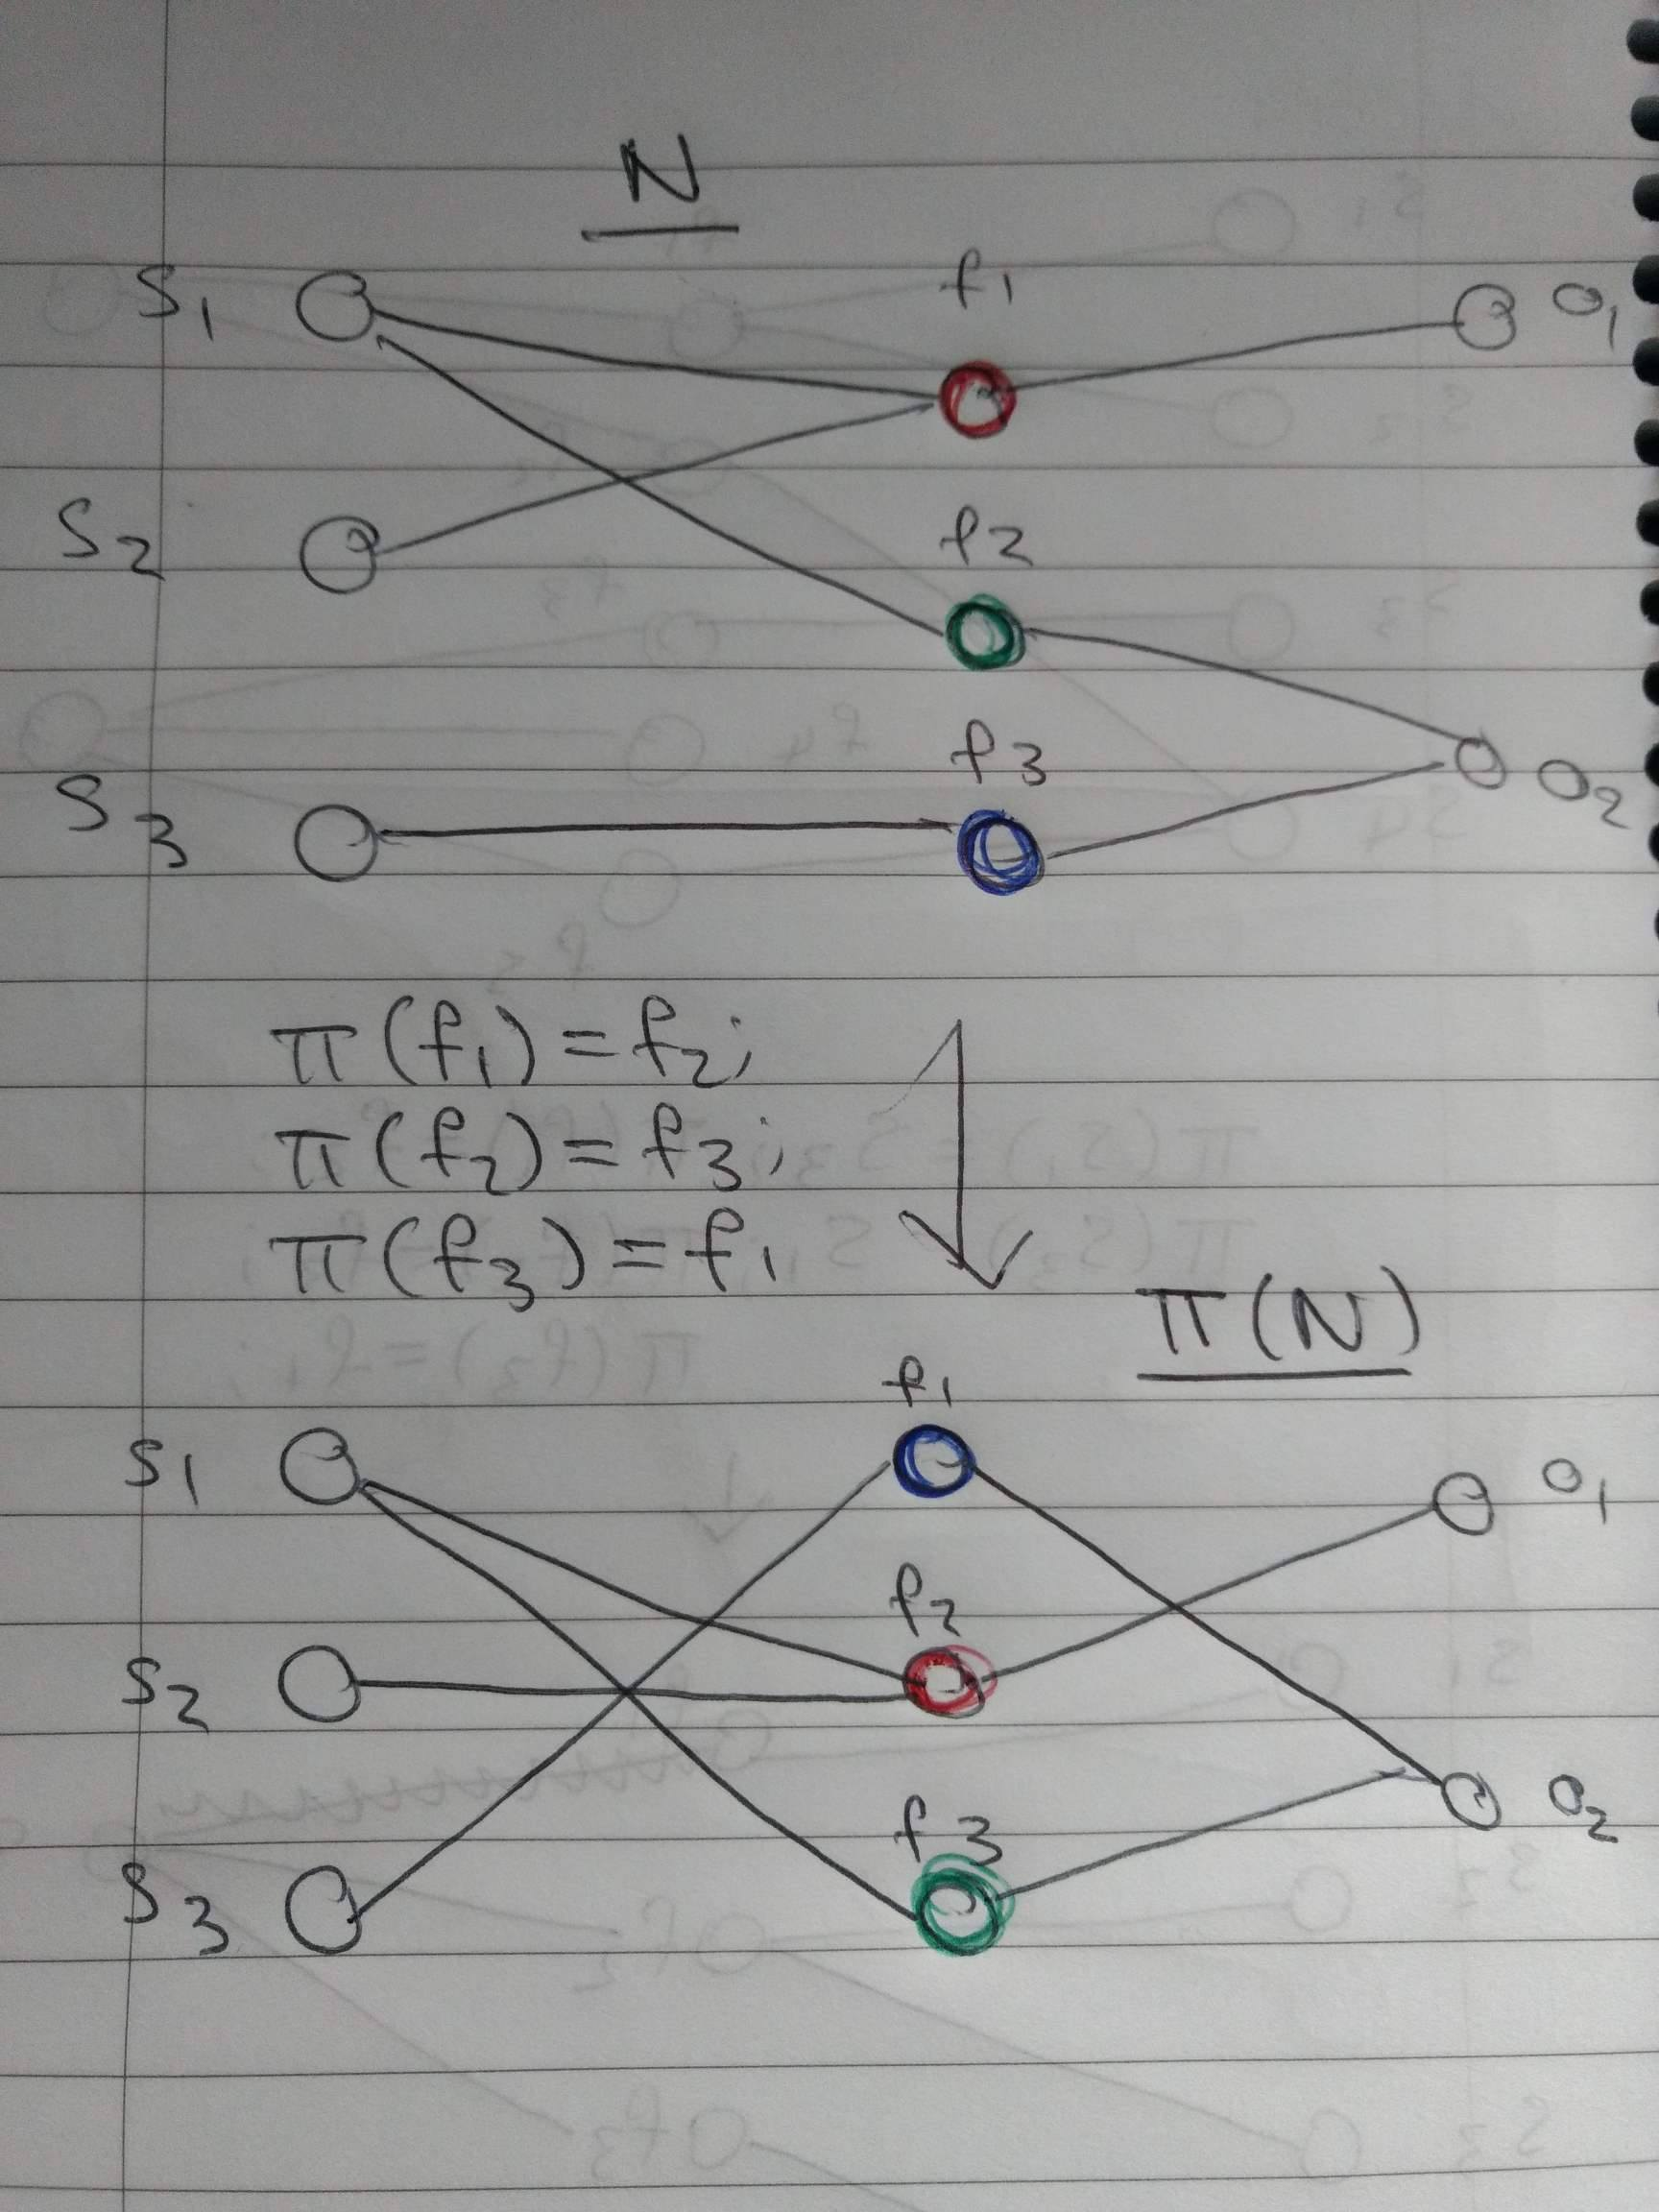
\includegraphics[width=\linewidth]{symmetry_example}
    \caption{
        Example of two equivalent truth discovery networks. Here the
        isomorphism between the left and right networks is $\pi = (S, T, U)(A,
        B)$. The colours show that the structure of the right network is the
        same as the left, just with different `names' for the nodes.
    }
    \label{img:equivalent_networks}
\end{figure}

\begin{proposition}
\label{prop:symm_iff_fact_source_object_symm}
$T$ satisfies symmetry if and only if it satisfies source, fact and object
symmetry.
\end{proposition}

\begin{proposition}
\label{prop:same_facts_ranked_equally}
If $T$ satisfies source-symmetry and $\fact(N, s_1) = \fact(N, s_2)$ in some
network $N$, then $s_1 \seq_N^T s_2$.

Similarly, if $T$ satisfies fact-symmetry and $\src(N, f_1) = \src(N, f_2)$,
$\obj(N, f_1) = \obj(N, f_2)$, then $f_1 \feq_N^T f_2$.

That is, any two sources making identical claims are ranked equally, and any
two facts for the same object with identical support from sources are ranked
equally.
\end{proposition}

All missing proofs are presented in the appendix.

In some sense the opposite of source-symmetry, where the identities of the
sources are irrelevant and only the structure of the truth discovery network is
important, is a situation where \emph{only} the identities of the sources are
considered.

\begin{definition}

A source $s^* \in \S$ is \emph{authoritative} for a network $N=(V, E)$ with
respect to an operator $T$ if $s \sle_N^T s^*$ for all $s \in S$, and $(s^*,
f^*) \in E$ implies $f \fle_N^T f^*$ for all $f \in \F$.

In other words, $s^*$ is more (or equally) trusted than all other sources, and
its facts are more (or equally) believable than all others.

We also define a strict version: $s^*$ is \emph{strictly authoritative} if
additionally $s \slt_N^T s^*$ for all $s \ne s^*$, and $f \flt_N^T f^*$ for all
$f, f^* \in \F$ such that $(s^*, f^*) \in E$ and $(s^*, f) \notin E$.

An operator $T$ is a \emph{dictatorship} if there is a source $s^* \in S$ (the
dictator) that is authoritative for all networks, and $T$ is a \emph{strict
dictatorship} if there is a source $s^* \in S$ that is strictly authoritative
for all networks.

\end{definition}

\begin{axiom}[Non-dictatorship]
\label{axiom:non_dict}
An operator $T$ should not be a dictatorship.
\end{axiom}

As noted above, source-symmetry and dictatorship are conceptually at odds with
one another. This is expressed formally in the following proposition, which
essentially shows that only trivial operators can satisfy both properties.

\begin{proposition}
\label{prop:symm_and_dict}

If an operator $T$ is both source-symmetric and a dictatorship, then for any
network $N$:
\begin{enumerate}
\item All sources are ranked equally
\item If $f_1$ is claimed by at least one source in $N$, then $f_2 \fle_N^T
f_1$ for all facts $f_2$.
\end{enumerate}

In particular, there is no operator that is both source-symmetric and a strict
dictatorship.
\end{proposition}

\begin{example}
A trivial operator that satisfies symmetry and dictatorship is one that always
ranks all sources and facts equally: $T_{triv}(N) = (\S^2, \F^2)$.

If we restrict $\N$ to those networks where all facts are claimed by
at least one source, then proposition \ref{prop:symm_and_dict} shows that $T$
satisfies source-symmetry and dictatorship if and only if $T=T_{triv}$.

Without this restriction, facts not claimed by any source may be ranked
strictly below other facts. Indeed, consider $T$ defined as follows. For any
network $N$ write $F_{+} = \{f \in \F : \src(N, f) \ne \emptyset \}$, and
define $T$ by $s_1 \seq_N^{T} s_2 \text{ for all } s_1, s_2 \in \S$, and
$$
    f_1 \fle_N^{T} f_2 \iff f_2 \in F_{+} \text{ or } f_1 \notin F_{+}
    \quad
    (f_1, f_2 \in \F)
$$

$T$ is trivially a dictatorship for \emph{any} $s^* \in \S$. It can be easily
checked that $\fle_N^T$ is a well-defined total preorder, and that $T$ is also
symmetric. However any fact in $\F \setminus F_+$ ranks strictly below any fact
in $F_+$.
\end{example}

Dictatorship requires there to be a fixed source that is authoritative
in all networks. A weaker form of dictatorship, which is more compatible with
symmetry, is where the authoritative source may depend on $N$.

\begin{definition}
\label{def:gen_dict}
A truth discovery operator $T$ is a \emph{generalised dictatorship} if for
every network $N$ there exists a source $s_N \in \S$ that is authoritative for
$N$ with respect to $T$. A \emph{generalised strict dictatorship} is defined
similarly.
\end{definition}

Clearly a dictatorship is also a generalised dictatorship.

\begin{example}
\label{example:symm_and_gen_dict}
An operator that is both symmetric and a generalised dictatorship is the
numerical operator $T$ defined as follows. For any truth discovery network $N$,
let $Q_N = \{s \in \S \colon |\fact(N, s)| = \max_{x \in \S}{|\fact(N, x)|}\}$
be the set of sources making the maximal number of claims, and set
\[
    t_N(s) = \begin{cases}
        1 & \text{ if } s \in Q_N \\
        0 & \text{ otherwise}
    \end{cases}
\]
\[
    b_N(f) = \begin{cases}
        1 & \text{ if } \src(N, f) \cap Q_N \ne \emptyset \\
        0 & \text{ otherwise}
    \end{cases}
\]
Clearly any source in $Q_N$ is authoritative.

To show symmetry, let $N$ and $\pi(N)$ be equivalent networks. Let $s \in \S$.
First note that $f \in \fact(N, s)$ iff $\pi(f) \in \fact(\pi(N), \pi(s))$ by
definition of equivalent networks, and in particular the restriction of $\pi$
to $\fact(N, s)$ is a bijection into $\fact(\pi(N), \pi(s))$; hence $|\fact(N,
s)| = |\fact(\pi(N), \pi(s))|$. Also, since $\pi$ restricted to $\S$ is a
bijection into $\S$, we have
\begin{align*}
    \max_{x \in \S}{|\fact(N, x)|} & = \max_{x \in \S}{|\fact(\pi(N), \pi(x))|} \\
                                   & = \max_{x \in \S}{|\fact(\pi(N), x)|}
\end{align*}
\begin{align*}
    s \in Q_N & \iff |\fact(N, s)| = \max_{x \in S}{|\fact(N, x)|} \\
              & \iff |\fact(\pi(N), \pi(s))| = \max_{x \in S}{|\fact(\pi(N), x)|} \\
              & \iff \pi(s) \in Q_{\pi(N)}
\end{align*}
We see that $t_N(s) = t_{\pi(N)}(\pi(s))$ for any $s \in \S$.

Now let $f \in \F$. Note that $s \in \src(N, f)$ iff $\pi(s) \in \src(\pi(N),
\pi(f))$. Using this fact and $s \in Q_N \iff \pi(s) \in Q_{\pi(N)}$, it is
easy to see that $\src(N, f) \cap Q_N \ne \emptyset$ iff $\src(\pi(N), \pi(f))
\cap Q_{\pi(N)} \ne \emptyset$, i.e. $b_N(f) = b_{\pi(N)}(\pi(f))$.

Finally this means, for any $s_1, s_2 \in \S$ and $f_1, f_2 \in \F$:
\begin{align*}
    s_1 \sle_N^T s_2 & \iff t_N(s_1) \le t_N(s_2) \\
                     & \iff t_{\pi(N)}(\pi(s_1)) \le t_{\pi(N)}(\pi(s_2)) \\
                     & \iff \pi(s_1) \sle_{\pi(N)}^T \pi(s_2)
\end{align*}
and similarly $f_1 \fle_N^T f_2$ iff $\pi(f_1) \fle_{\pi(N)}^T f_2$. Hence $T$
is symmetric.
\end{example}

Note that to be a generalised dictatorship, an operator needs only to rank
facts claimed by the most trusted source(s) above all other facts. One may
argue that this is not necessarily an undesirable property, since the most
trusted source presumably claims believable facts, which \emph{should} rank
highly.

However, the operator in example \ref{example:symm_and_gen_dict} has the
additional (perhaps undesirable) property that the ranking is `binary': it is
two-level ranking where all non-authoritative sources rank equally to each
other and strictly below the authoritative ones. This behaviour is captured in
the following definition.

\begin{definition}
A truth discovery operator $T$ is a \emph{binary generalised dictatorship} if
for every network $N$ there is a set of sources $Q_N \subseteq \S$ such that,
with
\begin{align*}
    t_N(s) & = \begin{cases}
        1 & \text{ if } s \in Q_N \\
        0 & \text{ otherwise}
    \end{cases} \\
    b_N(f) & = \begin{cases}
        1 & \text{ if } \src(N, f) \cap Q_N \ne \emptyset \\
        0 & \text{ otherwise}
    \end{cases}
\end{align*}
it holds that
\[ s_1 \sle_N^T s_2 \iff t_N(s_1) \le t_N(s_2) \]
\[ f_1 \fle_N^T f_2 \iff b_N(f_1) \le b_N(f_2) \]

\end{definition}

\begin{remark}
If $T$ is a binary generalised dictatorship, it clear that for each network
$N$, each source in $Q_N$ is authoritative.

In such case the orderings $\sle_N^T$ and $\fle_N^T$ are fully determined by
the choice of $Q_N$. Therefore a binary generalised dictatorship can be
identified with a mapping $\N \rightarrow 2^\S$ that selects the authoritative
sources for each truth discovery network.
\end{remark}

\begin{axiom}[Non- binary generalised dictatorship]
\label{axiom:non_bin_gen_dict}
An operator $T$ should not be a binary generalised dictatorship.
\end{axiom}

\begin{proposition}
\label{prop:non_dict_and_non_bin_gen_dict_indep}
Non-dictatorship and non- binary generalised dictatorship are independent.
\end{proposition}

\subsubsection{Unanimity}

The next axioms formalise the idea that if all sources are in agreement about
the status of a fact, then a truth discovery operator should respect this in
its verdict. Two obvious ways in which sources can be in agreement are when
\emph{all} sources believe a fact is true, and when \emph{no} sources believe a
fact is true.

\begin{axiom}[Unanimity]
\label{axiom:unanimity}
For any truth discovery network $N$, $\src(N, f) = \S$ implies $f' \fle_N^T f$
for all $f' \in \F$.
\end{axiom}

\begin{axiom}[Groundedness]
\label{axiom:groundedness}
For any truth discovery network $N$, $\src(N, f) = \emptyset$ implies $f
\fle_N^T f'$ for all $f' \in \F$.
\end{axiom}

That is, a fact cannot do better than to be claimed by all sources when $T$
satisfies unanimity, and cannot do worse than to be claimed by no sources when
$T$ is grounded.

Note that we do not require strict inequalities here, so as to not be too
restrictive. For unanimity in particular, requiring $f$ to rank strictly above
all other facts would require $T$ to choose a highest-ranking fact arbitrarily
in the case where there are multiple facts claimed by all sources.

Unanimity is similar to the \emph{weak Paretian} property \cite{handbook_intro}
in social choice, which states that whenever each individual prefers an
alternative $a$ over $b$, the social preference order prefers $a$ over $b$
also. It can also be compared to unanimity in judgement
aggregation \cite{handbook_ja}.

Axioms similar to groundedness have been proposed for collective annotation
(e.g. see \emph{groundedness} in \cite{kruger})

\todo{check social choice and JA incarnations of these principles}.

\begin{example}
The \emph{majority voting} operator, which ranks a fact by the number of
sources claiming it, satisfies unanimity and groundedness. Indeed, define
$T_{vote}$ by $s_1 \seq_N^{T_{vote}} s_2$ for all $s_1, s_2 \in \S$, and
    $$ f_1 \fle_N^{T_{vote}} f_2 \iff |\src(N, f_1)| \le |\src(N, f_2)| $$

If $\src(N, f) = \S$ then for all $f'$ we have $\src(N, f') \subseteq \S =
\src(N, f)$, so $f' \fle_N^T f$. Also, if $\src(N, f) = \emptyset$ then
$\src(N, f) \subseteq \src(N, f')$ for all $f'$, so $f \fle_N^T f'$. Hence
$T_{vote}$ is unanimous and grounded.
\end{example}

A consequence of groundedness is that any fact ranking strictly above all
others must have been claimed by at least one source (assuming $|\F|>1$).

\begin{proposition}
\label{prop:unam_ground_indep}
Unanimity and groundedness are independent.
\end{proposition}

\subsubsection{Independence}

In social choice, the `Independence of Irrelevant Alternatives' (IIA) axiom
\cite{arrow} requires that the relative ranking of two alternatives $A$ and $B$
depends only on the individual rankings of $A$ and $B$, and not on any
`irrelevant' alternative $C$. That is, if the individual voter preferences are
changed such that the ranking of $A$ versus $B$ remains the same for each
voter, the ranking of $A$ and $B$ in the social ranking remains unchanged.

\begin{figure}
    \centering
    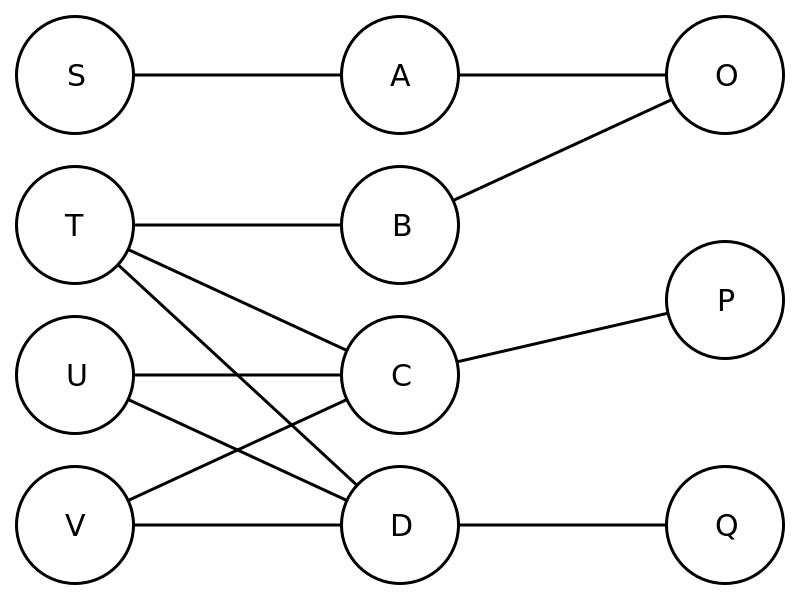
\includegraphics[width=25em]{independence_illustration_1}
    \caption{
        A network demonstrating a case where we do not wish for an IIA-type
        axiom to hold.
    }
    \label{img:independence_illustration_1}
\end{figure}

To consider whether a similar axiom should be adopted for truth discovery,
consider facts $A$ and $B$ in the network shown in figure
\ref{img:independence_illustration_1}. $A$ has support from source $S$ only,
who is not in agreement with any other sources, whilst $B$ has support from
$T$, who agrees with both $U$ and $V$ on facts $C$ and $D$. For this reason, it
may be reasonable to expect that $T$ is more trustworthy than $S$, and
therefore $B$ is more believable than $A$.

Directly translating IIA to this situation, we would require that the ranking
of $A$ and $B$ is unchanged if, say, we removed $T$'s claims for $C$ and $D$
(which are `irrelevant'), and instead had $S$ make these claims. However the
intuition above suggests that the ranking of $A$ and $B$ should actually be
\emph{reversed} in this case, despite the individual judgements on $A$ and $B$
remaining unchanged. For this reason, we argue that a more subtle notion of
independence is required.

\begin{figure}
    \centering
    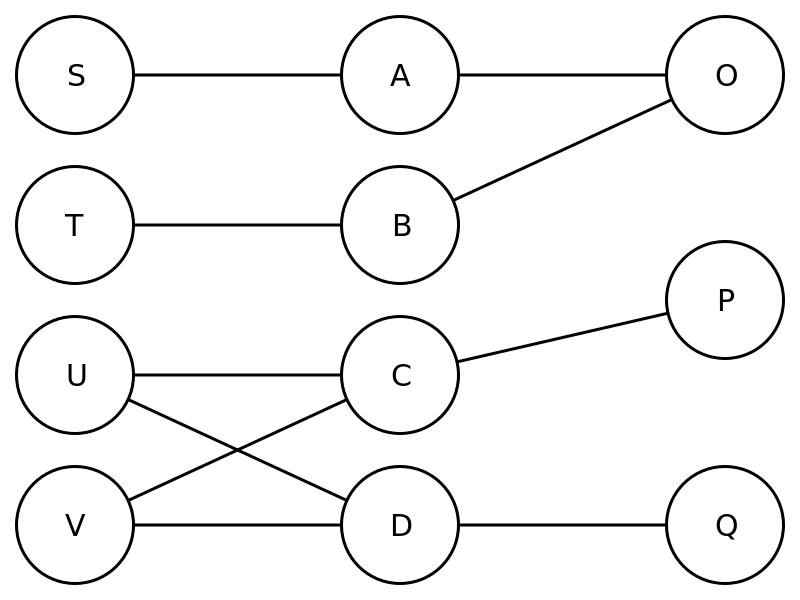
\includegraphics[width=25em]{independence_illustration_2}
    \caption{
        A network where some notion of independence may be applied
    }
    \label{img:independence_illustration_2}
\end{figure}

The issue in figure \ref{img:independence_illustration_1} is that $C$ and $D$
are not entirely irrelevant to $A$ and $B$, since they are connected indirectly
via sources that make claims for both objects $O$ and $P$ (namely, source $T$).
Consider removing these indirect links, as show in figure
\ref{img:independence_illustration_2}. In this case it can be argued that $C$
and $D$ truly are irrelevant to $A$ and $B$, and so changes to the network
outside of $S$, $T$, $A$, $B$ and $O$ should not affect the ranking of $A$ and
$B$.

This idea can be generalised by noting that two nodes are `relevant' to each
other (perhaps indirectly) if they lie in the same \emph{connected component}
of the network (where we consider the connected components of the undirected
version of the graph). A suitable independence axiom is therefore to require
that changes outside a connected component do not affect the ranking of sources
and facts within that component. A precise statement is given below.

\begin{axiom}[Independence Of Irrelevant Stuff]
\label{axiom:indep}
For any truth discovery networks $N_1$, $N_2$ with a common connected component
$G$, the restrictions of $\sle_{N_1}^T$ and $\sle_{N_2}^T$ to $G \cap \S$ are
equal, and the restrictions of $\fle_{N_1}^T$ and $\fle_{N_2}^T$ to $G \cap \F$
are equal.
\end{axiom}

Independence of irrelevant stuff requires that $s_1 \sle_{N_1}^T s_2$ if and
only if $s_1 \sle_{N_2}^T s_2$. A weaker version is to require only that the
ranking of $s_1$ and $s_2$ in $N_1$ is \emph{not reversed} in $N_2$, not
necessarily that the ranking if the same (for example, a strict inequality in
$N_1$ may become weak in $N_2$).

\begin{axiom}[Weak Independence Of Irrelevant Stuff]
\label{axiom:weak_indep}
For any truth discovery networks $N_1$, $N_2$ with a common connected component
$G$ and for any $s_1, s_2 \in G \cap S$ and $f_1, f_2 \in G \cap \F$:
\[
    s_1 \slt_{N_1}^T s_2 \implies s_1 \sle_{N_2}^T s_2
\]
\[
    f_1 \flt_{N_1}^T f_2 \implies f_1 \fle_{N_2}^T f_2
\]
\end{axiom}

Clearly axiom \ref{axiom:indep} implies axiom \ref{axiom:weak_indep}.

\subsubsection{Coherence}

A guiding principle of many truth discovery approaches is that facts claimed by
trustworthy sources should receive high belief, and sources claiming high
belief facts should be seen as trustworthy -- the trust and belief rankings
should cohere with one another in this sense. The following axiom aims to
formalise this in a specific case where it is possible to compare facts for two
sources in a straightforward way (and similarly for facts).

\begin{axiom}[Coherence]
Suppose $N$ is a truth discovery network and $s_1, s_2 \in \S$ are such that
there is a bijective mapping $\phi: \fact(N, s_1) \rightarrow \fact(N, s_2)$
with $f \fle_N^T \phi(f)$ for all $f \in \fact(N, s_1)$. Then $s_1 \sle_N^T
s_2$.

That is, if the facts claimed by two sources can be paired up such that the
fact claimed by $s_1$ always ranks beneath the fact claimed by $s_2$, then
$s_1$ ranks beneath $s_2$.

Similarly, if there are facts $f_1, f_2 \in \F$ and a bijection $\phi: \src(N,
f_1) \rightarrow \src(N, f_2)$ such that $s \sle_N^T \phi(s)$ for all $s \in
\src(N, f_1)$, then $f_1 \fle_N^T f_2$.

\end{axiom}

\todo{Come up with an example of a coherent operator}

\subsubsection{Monotonicity}

The axioms considered so far have largely dealt with the output of a truth
discovery operator for one input network at a time, or for two networks which
are structurally similar. Another dimension to the axiomatic approach is to
consider how the output of an operator is effected by a \emph{change} in the
input to modify it in a particular way.

The following axiom considers what should happen if a network is changed by
adding additional support for a particular fact. Intuitively, this should be
seen as additional evidence that the fact is true, and an operator should rate
it no worse than it did before.

\todo{
    expand introductory note: compare to monotonicity in social choice, JA,
    annotation, trust recommendation
}

\begin{axiom}[Monotonicity]
Let $N = (V, E)$ be a truth discovery network, and $f \in \F$, $s \in \S$ such
that $(s, f) \notin E$. Write $o = \obj(N, f)$. Consider the network $N'=(V,
E')$ where $s$ claims $f$, i.e.
$$
    E' = \{(s, f)\} \cup E \setminus \{(s, f') : f' \ne f, (f', o) \in E\}
$$
Then $f' \fle_N^T f$ implies $f' \fle_{N'}^T f$ for all $f' \in \F$.

That is, if $f$ receives additional support from a new source $s$, its ranking
should not get worse.
\end{axiom}

\todo{Come up with an example of a monotonic operator }

\todo{Summary of all the axioms and any implications between them}

\subsection{Iterative truth discovery operators}

Real-world algorithms for truth discovery generally compute numerical trust and
belief scores, as per definition \ref{def:numerical}. Additionally, most
operate in an \emph{iterative} manner, computing trust and belief scores
recursively from one another until the respective scores (hopefully) converge
to fixed values.

In this section we define the concept of iterative truth discovery operators to
represent and reason about such real-world algorithms.

\begin{definition}
\label{def:iterative_operator}

An \emph{iterative truth discovery operator} is a sequence $I=(T_n)_{n \in
\Nat}$ of numerical truth discovery operators, i.e. a sequence of mappings $T_n
: \N \rightarrow \R^\S \times \R^\F$.

For a network $N$ and $n \in \Nat$ we will write $T_n(N) = (t_N^n, b_N^n)$ to
refer directly to the source trust and claim belief mappings for the $n$-th
iteration (but note that this notation does not make explicit the dependence of
$t$ and $b$ on the sequence $I$).

$I$ is said to \emph{converge} to a numerical operator $T^*$ if $t_N^n
\rightarrow t_N^*$ and $b_N^n \rightarrow b_N^*$ pointwise as $n \rightarrow
\infty$ for each network $N$.

\end{definition}

\begin{remark}
Recall that a numerical operator $T^*$ naturally induces a (non-numerical)
operator by rankings sources according to $t_N^*$ and facts according to
$b_N^*$. We may therefore identify a convergent iterative operator $I$ with the
operator induced by its limit $T^*$, and write $\sle_N^I$ and $\fle_N^I$ for
the source and fact rankings. To be explicit:

$$ s_1 \sle_N^I s_2 \iff \lim_{n \rightarrow \infty}{t_N^n(s_1)} \le \lim_{n
\rightarrow \infty}{t_N^n(s_2)} $$

and similarly for facts.

Note that this mapping is not injective: there may be many iterative operators
with the same limit $T^*$; furthermore two distinct numerical operators $T^*$
and $T^{**}$ may induce the same non-numerical operator.
\end{remark}

Given a real-world algorithm in practise, one usually aims to determine whether
it converges by iterating until the distance (measured in some suitable way)
between trust (or belief) scores in consecutive iterations becomes smaller than
a fixed threshold. This is of course only a heuristic, since it is not possible
to determine whether a sequence converges by considering only finitely many
terms. Moreover even if the difference between subsequent trust/belief scores
were to become \emph{arbitrarily} small (i.e. smaller than \emph{any}
threshold), one still cannot guarantee convergence\footnotemark. This means
that it may not be trivial to define a real-world algorithm as a truth
discovery operator, since it may not be clear whether the trust and belief
scores converge in all cases. Nevertheless, in this work we will assume that
the iteration \emph{does} converge in all cases and consider which axioms of
section \ref{sec:axioms} are satisfied given this assumption.

\footnotetext{
    For an example of a sequence exhibiting such behaviour, consider the
    partial sums of the \emph{Harmonic series}
    $\sum_{j=1}^{\infty}\frac{1}{j}$, which is divergent. The difference
    between the $(n+1)$-th and $n$th terms is $\frac{1}{n+1}$ which converges
    to 0 as $n \rightarrow \infty$, yet the series does not converge.
}

To check whether a convergent operator satisfies the axioms, it will be
convenient to have sufficient conditions for some of the axioms that refer to
the numeric trust and belief scores directly.

For convenience we assume that trust and belief scores are in the range $[0,
1]$, as this is generally the case in practise.

\begin{lemma}
\label{lemma:iterative_axiom_suff_conds}
Let $I$ be a convergent iterative truth discovery operator with limit
$T^*$. Suppose that $t_N^n(s) \in [0, 1], b_N^n(f) \in [0, 1]$ for all $N, s,
f$ and $n$.

\begin{enumerate}
    \item $t_N^*(s) \in [0, 1]$ and $b_N^*(f) \in [0, 1]$

    \item If for any equivalent networks $N$ and $N'=\pi(N)$ it holds that
    \[
        t_N^n(s) = t_{\pi(N)}^n(\pi(s))
    \]
    and
    \[
        b_N^n(f) = b_{\pi(N)}^n(\pi(f))
    \]
    for all $N, n, s, f$, then $I$ satisfies symmetry (axiom \ref{axiom:symm}).

    \item If for any network $N$ and $f \in \F$,
    \[
        \src(N, f) = \S \implies b_N^n(f) = 1 \text{ for sufficiently large }
            n \in \Nat
    \]
    then $I$ satisfies unanimity (axiom \ref{axiom:unanimity}).

    \item If for any network $N$ and $f \in \F$,
    \[
        \src(N, f) = \emptyset \implies b_N^n(f) = 0
            \text{ for sufficiently large } n \in \Nat
    \]
    Then $I$ satisfies groundedness (axiom \ref{axiom:groundedness}).

    \item If for any networks $N_1$, $N_2$ with a common connected component
    $G$ it holds that $t_{N_1}^n(s) = t_{N_2}^n(s)$ and $b_{N_1}^n(f) =
    b_{N_2}^n(f)$ for $s \in G \cap \S$ and $f \in G \cap \F$, then $I$
    satisfies independence of irrelevant stuff (axiom \ref{axiom:indep}).

    \item If for any networks $N_1$, $N_2$ with a common connected component
    $G$ there are sequences of non-negative numbers $(\alpha_n)_{n \in \Nat}$,
    $(\beta_n)_{n \in \Nat}$ such that, for all $n \in \Nat$, $s \in G \cap \S$
    and $f \in G \cap \F$,
        \[ t_{N_2}^n(s) = \alpha_n \cdot t_{N_1}^n(s) \]
        \[ b_{N_2}^n(f) = \beta_n \cdot b_{N_1}^n(f) \]
    then $I$ satisfies weak independence of irrelevant stuff (axiom
    \ref{axiom:weak_indep}).

\end{enumerate}
\end{lemma}

\subsubsection{Sums}

Sums \cite{pasternack} is an iterative algorithm for truth discovery based on
the Hubs and Authorities \cite{kleinberg} algorithm for the ranking of web
pages based on the hyperlink structure of the web. The trust score for a source
at a given iteration is computed as the sum of the current belief scores of its
claimed facts, and the belief score for a fact is given by the sum of its
sources trust scores.

The trust/belief scores are normalised at each iteration by dividing by the
maximum score; this prevents the scores growing without bound to ensure
convergence.

\begin{definition}[Sums]
Sums is the iterative truth discovery operator $I_{sums}$ defined for any
network $N$ as follows, where we write $t_n$ for $t_N^n$ for brevity:
\[
    t_1(s) = \frac{1}{2}, \quad b_1(f) = \frac{1}{2}
\]
and for $n > 1$:
\begin{align*}
    \hat{t}_n(s) & = \sum_{f \in \fact(N, s)}{b_{n - 1}(f)} \\
    \hat{b}_n(f) & = \sum_{s \in \src(N, f)}{\hat{t}_n(s)} \\
    t_n(s) & = \frac{\hat{t}_n(s)}{\max\limits_{x \in \S}{\hat{t}_n(x)}} \\
    b_n(f) & = \frac{\hat{b}_n(f)}{\max\limits_{y \in \F}{\hat{b}_n(y)}}
\end{align*}

Note that $\hat{t}$ and $\hat{b}$ are only used to define $t$ and $b$, and are
not part of the definition of Sums itself.

If a source $s$ makes no claims in $N$ (i.e. $\fact(N, s) = \emptyset$), we
follow the convention that an empty sum is 0 and set $\hat{t}_N^n(s)=0$
(similar for a fact without sources).
\end{definition}

\begin{remark}
The normalisation ensures that trust and belief scores always lie in $[0, 1]$.
Note that any source that makes at least one claim has strictly positive trust
score for all $n$, and any fact with at least one source has strictly positive
belief score. Since any network $N$ must contain at least one claim, this
ensures that the maximum in the denominator for $t_n$ and $b_n$ is non-zero.
\end{remark}

\begin{theorem}
\label{theorem:sums_axioms}
If Sums is convergent, it satisfies symmetry (axiom \ref{axiom:symm}),
non-dictatorship (axiom \ref{axiom:non_dict}), unanimity (axiom
\ref{axiom:unanimity}), groundedness (axiom \ref{axiom:groundedness}) and
weak independence of irrelevant stuff (axiom \ref{axiom:weak_indep}).
\end{theorem}

\begin{figure}
    \centering
    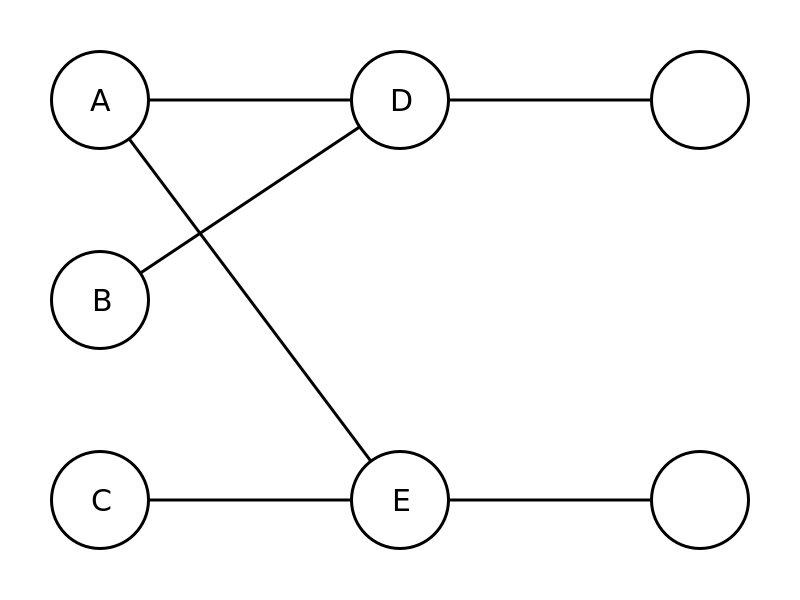
\includegraphics[width=25em]{sums_not_all_equal_trust}
    \caption{Network in which Sums does not rank all sources equally}
    \label{img:sums_not_all_equal_trust}
\end{figure}

The proof of theorem \ref{theorem:sums_axioms} uses lemma
\ref{lemma:iterative_axiom_suff_conds}, and can be found in the appendix. For
non-dictatorship, it is sufficient by proposition \ref{prop:symm_and_dict} and
symmetry to find a single truth discovery network in which Sums does not rank
all sources equally. Figure \ref{img:sums_not_all_equal_trust} shows such a
network: in this network $A$ ranks strictly above $B$ and $C$, which are ranked
equally.

\begin{theorem}
\label{theorem:sums_non_indep}
Sums does not satisfy Independence of Irrelevant Stuff (axiom
\ref{axiom:indep}).
\end{theorem}

\begin{figure}
    \centering
    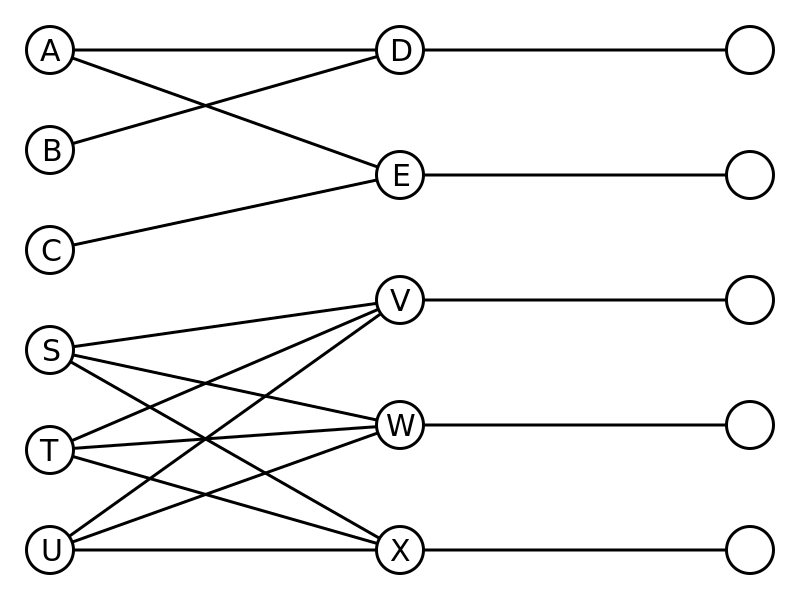
\includegraphics[width=25em]{sums_non_independence}
    \caption{
        Counter-example to independence for Sums: this network contains the one
        show in figure \ref{img:sums_not_all_equal_trust} as a connected
        component, but $A$ is ranked equal to $B$ here whereas it ranks
        strictly above $B$ in figure \ref{img:sums_not_all_equal_trust}.
    }
    \label{img:sums_non_indep}
\end{figure}

Figures \ref{img:sums_not_all_equal_trust} and \ref{img:sums_non_indep}
provide an example of Sums failing to satisfy independence. The details can be
found in the proof in the appendix.

We conjecture that Sums is indeed convergent for any input network. Indeed, it
is easy to see that Sums closely related to Hubs and Authorities
\cite{kleinberg}, where trust scores correspond to hub scores, and belief
scores correspond to authority scores. There are only two differences: the
initial scores ($\frac{1}{2}$ in Sums and 1 in Hubs and Authorities), and the
method of normalisation (Sums ensures the maximum score is 1, whereas Hubs and
Authorities ensures the sum of the squares of the scores is 1). In
\cite{kleinberg} is is proved that Hubs and Authorities always converges using
techniques from linear algebra. The difference in normalisation only amounts to
using a different norm to measure convergence (namely $\|.\|_{\infty}$ in Sums
instead of $\|.\|_2$), so it is hoped that the proof can be modified to work
for Sums.

\end{document}
